141. \begin{figure}[ht!]
\center{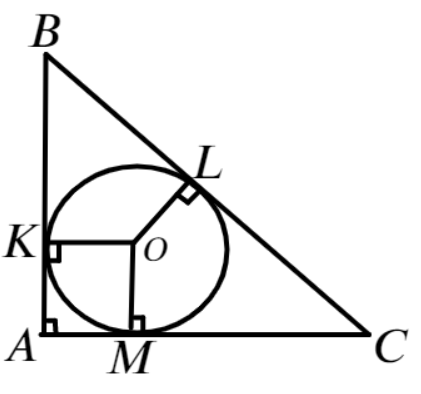
\includegraphics[scale=0.35]{g8-71.png}}
\end{figure}\\
Проведём радиусы к точкам касания. Так как отрезки касательных, проведённых из одной точки, равны, имеем $AK=AM,\ BK=BL,\ CL=CM.$ Так как $AKOM$ прямоугольник и $AK=AM,$ он является квадратом и радиус окружности тоже равен $AK.$ Пусть $AK=AM=x,$ тогда $AB=x+3,\ AC=x+2,\ BC=3+2=5$ и по теореме Пифагора для треугольника $ABC$ получаем $(x+3)^2+(x+2)^2=5^2,\ x^2+6x+9+x^2+4x+4=25,\ 2x^2+10x-12=0,\ x=1.$\\
